\chapter{Angular}\label{angular}

\section{Introduzione}

Lo scopo della pagina web prodotta in Angular, è quello di fornire le operazioni necessarie per attuare la modifica dello stato della lampada, sfruttando le funzionalità dell'API. \\
Nell'ottica del PoC, la modifica è riservata alla lampada con \texttt{id = 1}. \\
L'utente ha la capacità di visualizzare lo stato corrente della lampada, sia in forma visiva che testuale, e di modificarne lo stato. 

\section{Funzionamento}

\subsection{\texttt{lamp-button.component.ts}}
Questo componente consiste di un pulsante che cambia lo stato di una lampada. Visualizza inoltre un'immagine della lampada (Figura \ref{fig:getlamps}), variabile in base allo stato, e il suo stato corrente in forma testuale.

\subsection{All'avvio della pagina - \texttt{ngOnInit()}}
All'avvio della pagina web, viene invocato il metodo \texttt{getStatus()}.\\
Il metodo \texttt{getStatus()} è responsabile di ottenere lo stato corrente della lampada tramite una chiamata GET, ed aggiornare il valore locale nel BehaviorSubject \texttt{lampStatus\$} con il nuovo stato.

\subsection{\texttt{getStatus()}}
Questo metodo recupera lo stato corrente della lampada attraverso una chiamata GET all'endpoint (/lamps/1). \\

\subsection{Al tocco della lampada - \texttt{toggleLamp()}}

Si offre il metodo \texttt{toggleLamp()}, tale metodo cambia lo stato della lampada tramite una chiamata PUT, da un valore locale "On", ad "Off", e viceversa.

\section{Template HTML}
Il template HTML mostra un'immagine della lampada ed il suo stato corrente. \\
Tale immagine è anche un pulsante che chiama il metodo \texttt{toggleLamp()}, quando viene cliccata o premuta (Figura \ref{fig:modifylamps}).

\section{Metodi di supporto}

\subsection{\texttt{getData\$()}}
Si offre il metodo \texttt{getData\$()}, il quale effettua una richiesta HTTP GET all'endpoint API per recuperare lo stato corrente della lampada.

\subsection{\texttt{toggleLamp\$()}}
Questo metodo effettua una richiesta HTTP PUT all'endpoint API per cambiare lo stato della lampada. \\
Prende un parametro "status" che rappresenta lo stato corrente della lampada. \\
Se lo stato è "On", invia una modifica del parametro in "Off" per spegnere la lampada, e viceversa.

\section{Immagini}

\begin{figure}[H]
    \centering
    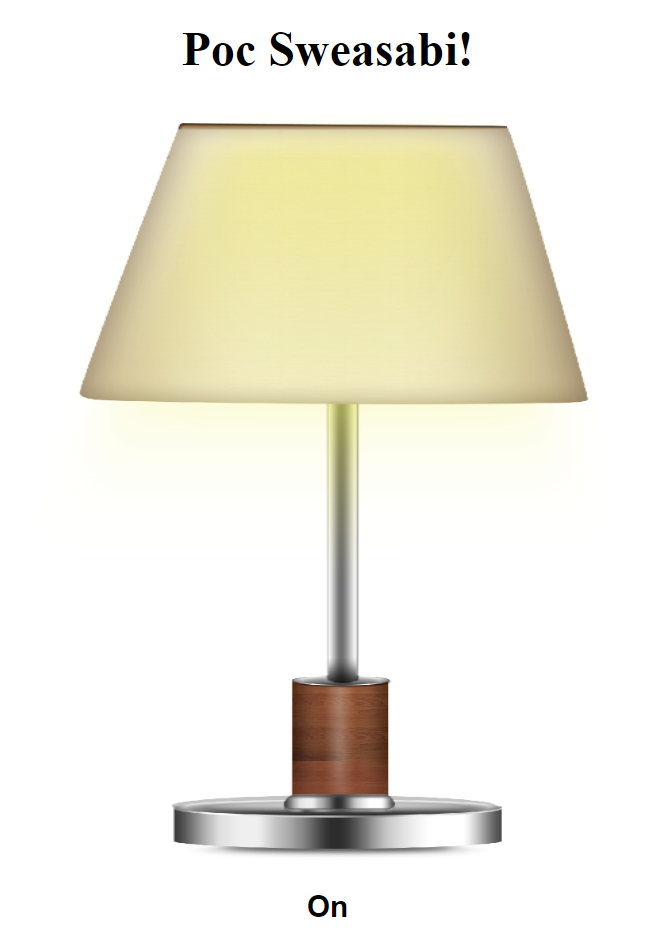
\includegraphics[width=0.5\linewidth]{getlamps.png}
    \caption{Button fa richiesta di stato iniziale su /Lamps/1}
    \label{fig:getlamps}
\end{figure}


\begin{figure}[H]
    \centering
    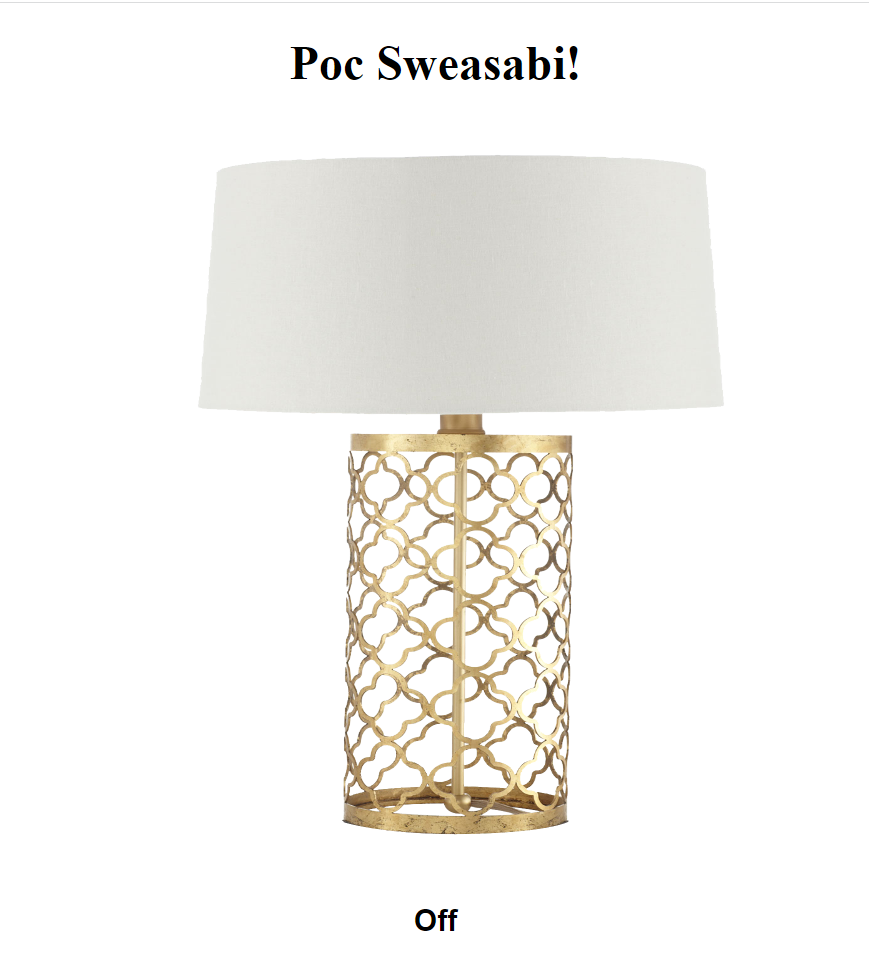
\includegraphics[width=0.6\linewidth]{modifylamps.png}
    \caption{Button fa cambio di stato su /Lamps/1}
    \label{fig:modifylamps}
\end{figure}